\documentclass[12pt,final,twoside]{report}
%%%%%%%%%%%%%%%%%%%%%%%%%%%%%%%%%%%%%%%%%%%%%%%%%%%%%%%%%%%%%
% Some credits:
% The template initially was created by Prof. Dr. Holger Karl/Uni Paderborn '2006
% and was expanded and updated by 
% - Stefan Heinrich/Uni Paderborn/Uni Hamburg since 2008,
% - Sven Magg/Uni Hamburg since 2013.
% Suggestions for changes are always welcome.
%%%%%%%%%%%%%%%%%%%%%%%%%%%%%%%%%%%%%%%%%%%%%%%%%%%%%%%%%%%%%
% Meta information:
\newcommand{\trtitle}{Compositional Generalization in Transformers}
\newcommand{\trtype}{Masterthesis} %{Bachelorthesis} %{Diplomarbeit} %{Dissertation}
\newcommand{\trcourseofstudies}{Intelligent Adaptive Systems} %{Bioinformatik} %{Intelligent Adaptive Systems} 
\newcommand{\trauthor}{Imran Ibrahimli}
\newcommand{\trauthordegree}{} %{\ B.Sc.}
\newcommand{\tremail}{imran.ibrahimli@studium.uni-hamburg.de}
\newcommand{\trmatrikelnummer}{7486484}
\newcommand{\trgutachterA}{\href{mailto:stefan.wermter@uni-hamburg.de}{Prof. Dr. Stefan Wermter}}
\newcommand{\trgutachterB}{\href{mailto:jae.hee.lee@uni-hamburg.de}{Dr. Jae Hee Lee}}
%\newcommand{\trbetreuung}{\href{mailto:tbd@informatik.uni-hamburg.de}{Dipl.-Inform. To Be Defined}}
\newcommand{\trfach}{Knowledge Technology, WTM}
\newcommand{\trdate}{24.10.2024}
\newcommand{\trkeywords}{Transformer, Algorithms, Mechanistic Interpretability}
%Optionally: it is also allowed to provide a street name on the
%\newcommand{\trstrasse}{Streetname 42}
%\newcommand{\trort}{22527 Hamburg}

%%%%%%%%%%%%%%%%%%%%%%%%%%%%%%%%%%%%%%%%%%%%%%%%%%%%%%%%%%%%%
% Languages:

% Falls die Ausarbeitung in Deutsch erfolgt:
% \usepackage[german]{babel}
% \usepackage[T1]{fontenc}
% \usepackage[latin1]{inputenc}
% \usepackage[latin9]{inputenc}                     
% \selectlanguage{german}

% If the thesis is written in English:
\usepackage[english]{babel}                         
\selectlanguage{english}

%%%%%%%%%%%%%%%%%%%%%%%%%%%%%%%%%%%%%%%%%%%%%%%%%%%%%%%%%%%%%
% Bind packages:
\usepackage{acronym}                    % Acronyms
\usepackage{algorithmic}                % Algorithms and Pseudocode
\usepackage{algorithm}                  % Algorithms and Pseudocode
\usepackage{amsfonts}                   % AMS Math Packet (Fonts)
\usepackage{amsmath}                    % AMS Math Packet
\usepackage{amssymb}                    % Additional mathematical symbols
\usepackage{amsthm}
\usepackage{booktabs}                   % Nicer tables
%\usepackage[font=small,labelfont=bf]{caption} % Numbered captions for figures
\usepackage{color}                      % Enables defining of colours via \definecolor
\definecolor{uhhRed}{RGB}{226,0,26}     % Official Uni Hamburg Red
\definecolor{uhhGrey}{RGB}{136,136,136} % Official Uni Hamburg Grey
\definecolor{uhhLightGrey}{RGB}{220, 220, 220}
\usepackage{fancybox}                   % Put equations in a frame
\usepackage{fancyhdr}                   % Packet for nicer headers
%\usepackage{fancyheadings}             % Nicer numbering of headlines
\usepackage[body={5.8in,9in}]{geometry} % Type area (size, margins...)

\geometry{a4paper,outer=3.35cm}        % !!!Release version (Normal margins)
%\geometry{a4paper,outer=2.5cm}         % !!!Print version (Additional margin on the left for the binding)
%\geometry{a4paper}                     % !!!Proofread version (Additional margin on the right for corrections)
% \geometry{a4paper,outer=3.134cm}        % !!!Draft version (Same margins on left and right)
%\geometry{paperheight=10.0in,paperwidth=6.4in,top=0.51in,left=0.3in}  % !!!Developer version (Minimal margins)

\usepackage{graphicx}                   % Inclusion of graphics
%\usepackage{latexsym}                  % Special symbols
\usepackage{longtable}                  % Allow tables over several parges
\usepackage{listings}                   % Nicer source code listings
\usepackage{multicol}                   % Content of a table over several columns
\usepackage{multirow}                   % Content of a table over several rows
\usepackage{rotating}                   % Alows to rotate text and objects
%\usepackage{siunitx}					% Nicer display of units and number according to SI standards
%\sisetup{tight-spacing=true}  
\usepackage[hang]{subfigure}            % Allows to use multiple (partial) figures in a fig
%HINT: subfigure may be depricated already - maybe try subfig instead 
%\usepackage[font=footnotesize,labelfont=rm]{subfig}    % Pictures in a floating environment
\usepackage{tabularx}                   % Tables with fixed width but variable rows
\usepackage{url,xspace,boxedminipage}   % Accurate display of URLs
\usepackage{csquotes}
\usepackage[citestyle=authoryear,bibstyle=authoryear,backend=biber]{biblatex}

\addbibresource{thesis.bib}


%%%%%%%%%%%%%%%%%%%%%%%%%%%%%%%%%%%%%%%%%%%%%%%%%%%%%%%%%%%%%
% PDF Information und Definitions:
\author{\trauthor}

\ifx\pdftexversion\undefined
\usepackage{hyperref}
\else
\usepackage[colorlinks=false,           % link is colores (true) or has colored frame (false)
            linkcolor=uhhRed,           % case colorlinks=true: define color.
            urlcolor=uhhRed,
            citecolor=uhhRed,
            bookmarks,                  % Place bookmarks erstellen
            bookmarksopen=true,         % Bookmarks will be shown at start (true/false)
            pdfpagemode=UseOutlines,    
            bookmarksopenlevel=1,       % Define the depth of shown links
            bookmarksnumbered,          % Numbers of chapers in Bookmarks
            pdftitle={\trtitle},
            pdfsubject={\trtype},
            pdfkeywords={\trkeywords},
            pdfauthor={\trauthor},
            plainpages=false
            ]{hyperref}
\fi

\ifx\pdftexversion\undefined
\else
\pdfoutput=1                            % Disable PDF-Output
\pdfimageresolution=1200
\pdfcompresslevel=2                     % 0 = no compression, 9 = strongest compression
\fi

%%%%%%%%%%%%%%%%%%%%%%%%%%%%%%%%%%%%%%%%%%%%%%%%%%%%%%%%%%%%%
% Configurationen:

\hyphenation{whe-ther}                  % Manually use: "\-" in a word: Staats\-ver\-trag

%\lstloadlanguages{C}                   % Set the default language for listings
\DeclareGraphicsExtensions{.pdf,.svg,.jpg,.png,.eps} % first try pdf, then eps, png and jpg
\graphicspath{{./img/}}                 % Path to a folder where all pictures are located
\pagestyle{fancy}                       % Use nicer header and footer

% Redefine the environments for floating objects:
\setcounter{topnumber}{3}
\setcounter{bottomnumber}{2}
\setcounter{totalnumber}{4}
\renewcommand{\topfraction}{0.9}        %Standard: 0.7
\renewcommand{\bottomfraction}{0.5}     %Standard: 0.3
\renewcommand{\textfraction}{0.1}       %Standard: 0.2
\renewcommand{\floatpagefraction}{0.8}  %Standard: 0.5

% Tables with a nicer padding:
\renewcommand{\arraystretch}{1.2}

% Chapter and Sections will not be written in capitals
\renewcommand{\chaptermark}[1]{\markboth{\chaptername \ \thechapter.\ #1}{}}
\renewcommand{\sectionmark}[1]{\markright{\thesection.\ #1}}

% Avoid french spacing (double spacing after a full stop)
\frenchspacing

%%%%%%%%%%%%%%%%%%%%%%%%%%%%
% Additional 'theorem' and 'definition' blocks:
\theoremstyle{plain}
\newtheorem{theorem}{Theorem}[chapter]
%\newtheorem{theorem}{Satz}[chapter]    % Wenn in Deutsch geschrieben wird.
\newtheorem{axiom}{Axiom}[chapter]     
%\newtheorem{axiom}{Fakt}[chapter]      % Wenn in Deutsch geschrieben wird.
%Usage:%\begin{axiom}[optional description]%Main part%\end{fakt}

\theoremstyle{definition}
\newtheorem{definition}{Definition}[chapter]

%Additional types of axioms:
\newtheorem{lemma}[axiom]{Lemma}
\newtheorem{observation}[axiom]{Observation}

%Additional types of definitions:
\theoremstyle{remark}
%\newtheorem{remark}[definition]{Bemerkung} % Wenn in Deutsch geschrieben wird.
\newtheorem{remark}[definition]{Remark} 

%%%%%%%%%%%%%%%%%%%%%%%%%%%%
% Provides TODOs within the margin:
\newcommand{\TODO}[1]{\marginpar{\emph{\textcolor{red}{\small{{\bf TODO: } #1}}}}}

%%%%%%%%%%%%%%%%%%%%%%%%%%%%
% Abbreviations and mathematical symbols
\newcommand{\modd}{\text{ mod }}
\newcommand{\RS}{\mathbb{R}}
\newcommand{\NS}{\mathbb{N}}
\newcommand{\ZS}{\mathbb{Z}}
\newcommand{\dnormal}{\mathit{N}}
\newcommand{\duniform}{\mathit{U}}

\newcommand{\erdos}{Erd\H{o}s}
\newcommand{\renyi}{-R\'{e}nyi}
% it is recommented to define complex terms as expression/newcommand and use the expression in the tex instead.

%%%%%%%%%%%%%%%%%%%%%%%%%%%%%%%%%%%%%%%%%%%%%%%%%%%%%%%%%%%%%
% Document:

\begin{document}

\pagenumbering{Roman}                   % Roman pagenumbering for lists and meta pages
\renewcommand{\headheight}{14.5pt}      % Size of headings

\thispagestyle{empty}
\fancyhead[LO,RE]{}                     % Define the header style for the meta pages

%%%%%%%%%%%%%%%%%%%%%%%%%%%%
% Cover sheet

\begin{titlepage}
  %---Possibility 1:
  \begin{flushleft}
    
\includegraphics[width=67mm]{uhhLogoL.pdf}\\
  \end{flushleft}
  \rule{\textwidth}{0.4pt}
  \newline
  \vspace{2.0cm}
  \begin{center}
    \LARGE \textbf{\trtitle}
  \end{center}
  \vspace{2.0cm}
  \begin{center}
    \textbf{\trtype}\\
    %im Arbeitsbereich \trfach\\
    at Research Group \trfach\\
    \trgutachterA\medskip\\
    %Fachbereich Informatik\\
    Department of Informatics\\
    %MIN-Fakult\"at\\
    MIN-Faculty\\
    Universit\"at Hamburg \\[1.0cm] %not allowed to translate Universit{\"a}t Hamburg
    %vorgelegt von \\
    submitted by \\
    \textbf{\href{mailto:\tremail}{\trauthor\trauthordegree}}\\
    %Studiengang:   \trcourseofstudies \\
    Course of study:   \trcourseofstudies \\
    Matrikelnr.:  \trmatrikelnummer \\
    %a\\
    on\\
    \trdate
  \end{center}
  \vspace{2cm}
  \begin{center}
    \begin{tabular}{ll}
      %Gutachter: & \trgutachterA \\
      Examiners: & \trgutachterA \\
                 & \trgutachterB \\
      %Betreuung: & \trbetreuung \\    	% Adviser are not allowed to demand getting mentioned here, but are happy getting credited by student's initiative
    \end{tabular}
  \end{center}
  \vfill
  %    \begin{tabular}{l}
  %    \trauthor \\
  %    Matrikelnummer:  \trmatrikelnummer \\
  %    \trstrasse \\
  %    \trort
  %    \end{tabular}
  %    \newline
  \rule{\textwidth}{0.4pt}
  \newpage
\end{titlepage}

%backsite of cover sheet is empty!
\thispagestyle{empty}
\hspace{1cm}
\newpage

%%%%%%%%%%%%%%%%%%%%%%%%%%%%
% Abstract:
\section*{Abstract}\label{sec:abstract}
%\fancyhead[LE,RO]{\it Abstract}
%\addcontentsline{toc}{chapter}{\numberline{}Abstract}
Your English abstract here (mandatory if written in English and recommended otherwise).

% If the abstract ist not longer than half a page, then the German Zusammenfassung can be places on the same page
%\cleardoublepage
\vfill
\section*{Zusammenfassung}\label{sec:zusammenfassung}
%\addcontentsline{toc}{chapter}{\numberline{}Zusammenfassung} %Add the Zusammenfassung to the TOC
Hier die deutsche Zusammenfassung einf\"ugen (notwendig).
\fancyhead[LE,RO]{\it Abstract}

\cleardoublepage

%%%%%%%%%%%%%%%%%%%%%%%%%%%%
% Lists:
%\setcounter{tocdepth}{1}               % depth of the table of contents (for BSc and MSc Thesis 1 is recommented)
\fancyhead[LE,RO]{\it Contents}
\tableofcontents
\cleardoublepage
% List of Figures and List of tables are optional. -> Not needed in most theses.
\fancyhead[LE,RO]{\it List of Figures}
\listoffigures
\cleardoublepage
\fancyhead[LE,RO]{\it List of Tables}
\listoftables
\cleardoublepage
%\lstlistoflistings
%\cleardoublepage

\fancyhead[LE]{\it \leftmark}           % Define the header style for the text pages
\fancyhead[RO]{\it \rightmark}          % Define the header style for the text pages
\fancyhead[LO,RE]{}                     % Define the header style for the text pages

%%%%%%%%%%%%%%%%%%%%%%%%%%%%
% The content will be included here:
\pagenumbering{arabic}

\chapter{Introduction}\label{introduction}



An Introduction usually is used only to provide a background, a motivation and a short readers guide. In this document it is used to reproduce some information about writing a thesis and writing in \LaTeX. To get started, just delete this content and start writing your own.

\section{How to Organize your Thesis}
In this section some revision of a generic structure of a thesis will be given. Please note that the complete text can be found on:
\begin{quote}
	http://www.sce.carleton.ca/faculty/chinneck/thesis.html
\end{quote}
Translations to other languages are available too:
\begin{quote}
	http://www.sce.carleton.ca/faculty/chinneck/thesis/translations.html
\end{quote}


\subsection{Introduction}

This is a general introduction to what the thesis is all about -- it is not just a description of the contents of each section. Briefly summarize the question (you will be stating the question in detail later), some of the reasons why it is a worthwhile question, and perhaps give an overview of your main results. This is a birds-eye view of the answers to the main questions answered in the thesis (see above).

\subsection{Background Information (optional)}

A brief section giving background information may be necessary, especially if your work spans two or more traditional fields. That means that your readers may not have any experience with some of the material needed to follow your thesis, so you need to give it to them. A different title than that given above is usually better; e.g., 'A Brief Review of Frammis Algebra.'

\subsection{Review of the State of the Art}

Here you review the state of the art relevant to your thesis. Again, a different title is probably appropriate; e.g., 'State of the Art in Zylon Algorithms.' The idea is to present (critical analysis comes a little bit later) the major ideas in the state of the art right up to, but not including, your own personal brilliant ideas.

You organize this section by idea, and not by author or by publication. For example if there have been three important main approaches to Zylon Algorithms to date, you might organize subsections around these three approaches, if necessary:
\begin{itemize}
	\item[3.1] Iterative Approximation of Zylons
	\item[3.2] Statistical Weighting of Zylons
	\item[3.3] Graph-Theoretic Approaches to Zylon Manipulation
\end{itemize}

\subsection{Research Question or Problem Statement}

Engineering theses tend to refer to a 'problem' to be solved where other disciplines talk in terms of a 'question' to be answered. In either case, this section has three main parts:

\begin{enumerate}
	\item a concise statement of the question that your thesis tackles
	\item justification, by direct reference to section 3, that your question is previously unanswered
	\item discussion of why it is worthwhile to answer this question.
\end{enumerate}

Item 2 above is where you analyze the information which you presented in Section 3. For example, maybe your problem is to 'develop a Zylon algorithm capable of handling very large scale problems in reasonable time' (you would further describe what you mean by 'large scale' and 'reasonable time' in the problem statement). Now in your analysis of the state of the art you would show how each class of current approaches fails (i.e. can handle only small problems, or takes too much time). In the last part of this section you would explain why having a large-scale fast Zylon algorithm is useful; e.g., by describing applications where it can be used.

Since this is one of the sections that the readers are definitely looking for, highlight it by using the word 'problem' or 'question' in the title: e.g. 'Research Question' or 'Problem Statement', or maybe something more specific such as 'The Large-Scale Zylon Algorithm Problem.'

\subsection{Description of How You Solved the Problem or Answered the Question}

This part of the thesis is much more free-form. It may have one or several sections and subsections. But it all has only one purpose: to convince the examiners that you answered the question or solved the problem that you set for yourself in Section 4. So show what you did that is relevant to answering the question or solving the problem: if there were blind alleys and dead ends, do not include these, unless specifically relevant to the demonstration that you answered the thesis question.

\subsection{Conclusions}

You generally cover three things in the Conclusions section, and each of these usually merits a separate subsection:

\begin{enumerate}
	\item Conclusions
	\item Summary of Contributions
	\item Future Research
\end{enumerate}

Conclusions are not a rambling summary of the thesis: they are short, concise statements of the inferences that you have made because of your work. It helps to organize these as short numbered paragraphs, ordered from most to least important. All conclusions should be directly related to the research question stated in Section 4. Examples:

\begin{enumerate}
	\item The problem stated in Section 4 has been solved: as shown in Sections ? to ??, an algorithm capable of handling large-scale Zylon problems in reasonable time has been developed.
	\item The principal mechanism needed in the improved Zylon algorithm is the Grooty mechanism.
	\item Etc.
\end{enumerate}

The Summary of Contributions will be much sought and carefully read by the examiners. Here you list the contributions of new knowledge that your thesis makes. Of course, the thesis itself must substantiate any claims made here. There is often some overlap with the Conclusions, but that's okay. Concise numbered paragraphs are again best. Organize from most to least important. Examples:

\begin{enumerate}
	\item Developed a much quicker algorithm for large-scale Zylon problems.
	\item Demonstrated the first use of the Grooty mechanism for Zylon calculations.
	\item Etc.
\end{enumerate}

The Future Research subsection is included so that researchers picking up this work in future have the benefit of the ideas that you generated while you were working on the project. Again, concise numbered paragraphs are usually best. 

\subsection{Appendices}

What goes in the appendices? Any material which impedes the smooth development of your presentation, but which is important to justify the results of a thesis. Generally it is material that is of too nitty-gritty a level of detail for inclusion in the main body of the thesis, but which should be available for perusal by the examiners to convince them sufficiently. Examples include program listings, immense tables of data, lengthy mathematical proofs or derivations, etc. 

\subsection{Bibliography}

The list of references is closely tied to the review of the state of the art given in section 3. Most examiners scan your list of references looking for the important works in the field, so make sure they are listed and referred to in section 3. Truth be known, most examiners also look for their own publications if they are in the topic area of the thesis, so list these too. Besides, reading your examiner's papers usually gives you a clue as to the type of questions they are likely to ask.

All references given must be referred to in the main body of the thesis. Note the difference from a Bibliography, which may include works that are not directly referenced in the thesis. Organize the list of references either alphabetically by author surname (preferred), or by order of citation in the thesis. 



\section{Revision: Writing in \LaTeX}
As thought in the seminars, \LaTeX is quite useful for writing a paper or a thesis. Nevertheless it comes with its own rules.

\subsection{Word processing with \LaTeX}
\label{sec:model:subsec:latex}

This document has already introduced the most important constructs of
\LaTeX. What is necessary to produce documents with \LaTeX is simple
any normal text editor and a \LaTeX distribution. This is commonly
installed on practically all UNIX-type systems; for Windows, an
excellent \LaTeX exists, called MikTeX, available from
\url{www.miktex.org}. Almost all distributions come with a large patch
of examples and introductory material; consult your local installation
for details. 

Lots of supplementary and background information, FAQs, etc.\ is
available from the Comprehensive TeX Archive Network (CTAN); the
German mirror of which is \url{www.dante.de}. 

\subsection{Tables in \LaTeX}
\label{sec:model:subsec:tables}
The table should be centred and should always have a caption positioned above it. A caption in a sentence form as well as in a short form must end with a period as seen in table~\ref{tab:sample}. Ideally the table can be understood sorely by the table and the caption itself. The parameters ``hbtp'' provide a list of priorities for the arrangement of the table: here, bottom, top, (next) page.

\begin{table}[hbtp]
	\caption{This caption has one line so it is centered.}\label{tab:sample}
	\centering
	\begin{tabular}{|c|c|}
		\hline
		Example column 1 & Example column 2 \\
		\hline
		Example text 1   & Example text 2   \\
		\hline
	\end{tabular}
\end{table}

\subsection{Figures in \LaTeX}
\label{sec:model:subsec:figures}
Note that a figure is a so-called floating object: it is moved around the actual text in order to best fit on a page. This is in strong contrast to some GUI-based word processing tools, where the placement of figures is usually more associated with luck than principle.

As figures float around, expressions like ``the following figure'' must never be used. Instead, figures need a caption, a label, and must be properly referenced in the main text. A figure caption is placed centred below the figure and describes the figure in (very) short. Again, ideally the figure can be understood sorely by the figure and the caption itself.

In general, only vector graphics in encapsulated postscript (EPS) or a similar format (SVG, PDF) should be included in any kind of text, as this allows arbitrary scaling, rotation etc.\ without any loss of quality. Bitmap formats (JPEG, GIF, \dots) should only be used if no other alternative exists --- basically the only case where bitmaps can be justified is when scanned pictures need to be included in a text, however, this should be avoided as hard as possible as the quality in usually not satisfactory. If a screen shot is needed a high resolution picture without visible fragments of a jpeg compression is allowed. Figures like the figure~\ref{fig:samplefig} (this is how you refer to figures correctly! the tilde is used as a non-breaking space) should always appear after the first referencing it.
\begin{figure}[hbtp]
	\centerline{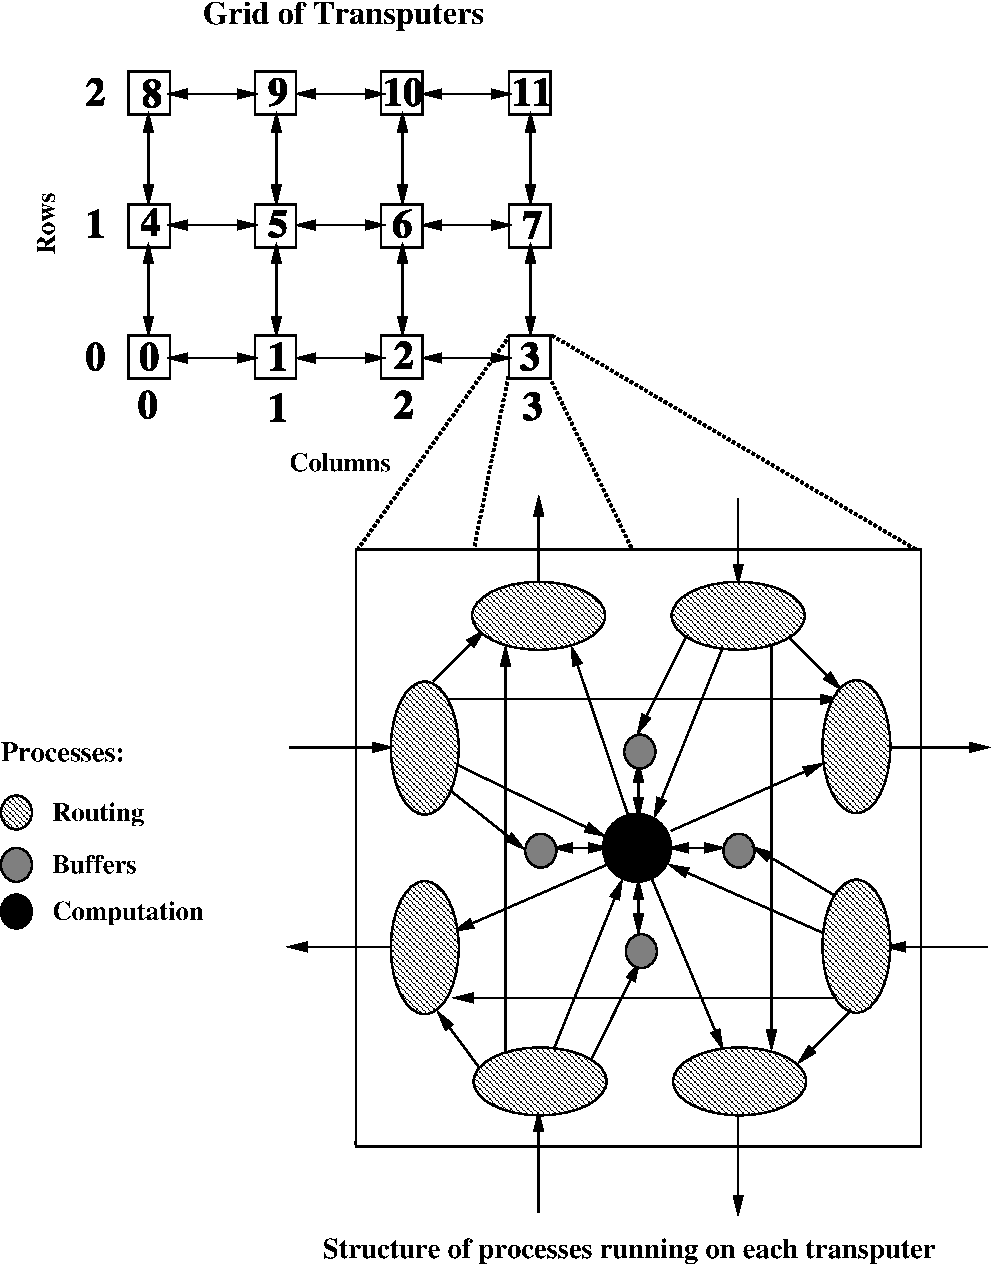
\includegraphics[width=0.6\textwidth]{samplefig.pdf}}
	{\caption{Network of transputers and the structure of individual
			processes.}\label{fig:samplefig}}
\end{figure}
\cleardoublepage

\chapter{Background}\label{background}

\TODO{rewrite}

This chapter provides an overview of the Transformer architecture, focusing on its core components, different variants, positional encoding schemes, and the processes of training and inference. It also discusses mechanistic interpretability and the deep double descent phenomenon.

\section*{Notation}\label{sec:notation}

\begin{center}
    \begin{tabular}{cl}
        $\mathcal{V}$ \qquad & Vocabulary (set) of input tokens.                                           \\
        $n$                  & Length of the input sequence.                                               \\
        $b$                  & Batch size for batched input sequences.                                     \\
        $\mathbf{x}$         & Input sequence of tokens, $\mathbf{x} \in \mathcal{V}^{n}$                  \\
        $x_i$                & $i$-th token in the input sequence, $x_i \in \mathcal{V}$.                  \\
        $d$                  & Dimensionality of the token embedding space.                                \\
        $E_i$                & $d$-dimensional embedding vector of token $x_i$, $E_i \in \mathbb{R}^d$.    \\
        $E$                  & Embedding matrix, $E \in \mathbb{R}^{|\mathcal{V}| \times d}$.              \\
        $H$                  & Matrix of a sequence of embedding vectors, $H \in \mathbb{R}^{n \times d}$. \\
        $H_i$                & $i$-th vector in the sequence of embeddings, $H_i \in \mathbb{R}^d$.        \\
        $O$                  & Output matrix from a Transformer layer, $O \in \mathbb{R}^{n \times d}$.    \\
        $Q$                  & Queries matrix, $Q \in \mathbb{R}^{n \times d}$.                            \\
        $K$                  & Keys matrix, $K \in \mathbb{R}^{n \times d}$.                               \\
        $V$                  & Values matrix, $V \in \mathbb{R}^{n \times d}$.                             \\
        $\theta$             & Model parameters (weights and biases).                                      \\
    \end{tabular}
\end{center}

\section{Transformer}\label{sec:transformer_arch}

The Transformer architecture, introduced by \textcite{vaswani_attention_2017}, performs sequence modeling by relying entirely on self-attention mechanism, instead of using convolution or recurrence.

Let $\mathcal{V}$ denote the vocabulary of input tokens. While the tokens can represent anything, in language modeling tasks they are usually learned subword units. In this work, however, a simple character tokenization scheme is used that is suitable for algorithmic tasks, so each token corresponds to a single character (letter, digit or symbol) in the sequence. An input sequence is represented as $\mathbf{x} = [x_1, x_2, \dots, x_n]$, where $x_i \in \mathcal{V}$ and $n$ is the sequence length. Each token $x_i$ is mapped to a $d$-dimensional embedding vector $E_i \in \mathbb{R}^d$ using an embedding matrix $E \in \mathbb{R}^{|\mathcal{V}| \times d}$. Thus, each row of $E$ corresponds to the embedding of a token in the vocabulary.

The input matrix to a Transformer layer is a sequence of vector embeddings (also called the \emph{latent} or \emph{hidden representation} for intermediate layer inputs), denoted $H \in \mathbb{R}^{n \times d}$, where $H = [H_1^\top, H_2^\top, \dots, H_n^\top]^\top$. The output of a Transformer layer is also a sequence of vectors with the same sequence length, denoted $O \in \mathbb{R}^{n \times d}$.

In practice, the inputs to the Transformer are batched, so the input has an additional dimension for the batch size, denoted $b$, with $H \in \mathbb{R}^{b \times n \times d}$. This results in the first (batch) dimension being added throughout the intermediate representation and the output, but has no bearing on the description of the Transformer model.

\subsection{Elements}\label{subsec:elements_transformers}

The Transformer is composed of several key components to model dependencies in sequential data: multi-head attention, feed-forward networks, layer normalization, and residual connections. Informally, the attention mechanism transfers information \emph{between} tokens, while the feed-forward networks process information \emph{within} tokens. These components are stacked in each layer of the Transformer as shown in Figure \ref{fig:transformer_layer} (a).

\paragraph{Token Embeddings}
The discrete input tokens are first converted into continuous embeddings using an embedding matrix $E \in \mathbb{R}^{|\mathcal{V}| \times d}$, where $|\mathcal{V}|$ is the size of the vocabulary and $d$ is the embedding dimension. The embedding matrix is learned during training, and the embeddings are used as input to the Transformer. After applying the Transformer layers, the output embeddings are passed through a linear \emph{unembedding} layer to get the \emph{logits} (unnormalized log-probabilities) for the next token.

\paragraph{Attention Mechanism}
The attention mechanism \parencite{bahdanau_neural_2014} allows the model to weigh the relevance of different positions in the input sequence. For this purpose, it computes \emph{queries}, \emph{keys}, and \emph{values} from the input embeddings and uses them to calculate attention scores. The output is a weighted sum of the values, where the weights are determined by the attention scores. The names ``queries'', ``keys'', and ``values'' are derived from the context of information retrieval, where the queries are the elements being searched for, the keys are the elements being searched, and the values are the elements being retrieved. In the context of the Transformer, intuitively, the query represents what the current token is ``looking for'' in the sequence, the keys represent what the token at a given position ``offers'' to the current token, and the values are the actual information that the current token ``receives'' from the other tokens.

First, the queries, keys, and values are computed as:
\begin{align*}
    Q & = H W^Q, \\
    K & = H W^K, \\
    V & = H W^V,
\end{align*}
where $W^Q, W^K, W^V \in \mathbb{R}^{d \times d_k}$ are the weight matrices, and $d_k$ is the dimension of the queries, keys, and values. In practice, the convention is to set $d_k = d$, which is the case for the models in this work. Thus, $Q, K, V \in \mathbb{R}^{n \times d}$.

Given queries $Q$, keys $K$, and values $V$, the attention output is computed as:
\begin{equation*}
    O_{att} = \text{Attention}(Q, K, V) = \text{softmax}\left( \frac{Q K^\top}{\sqrt{d}} \right) V.
\end{equation*}
where the softmax function is applied along the last dimension, and is defined as:
\begin{equation*}
    \text{softmax}(\mathbf{x})_i = \frac{e^{x_i}}{\sum_j e^{x_j}}.
\end{equation*}

Note that the output of the attention mechanism has the same shape as the input, $O_{att} \in \mathbb{R}^{n \times d}$.

\paragraph{Multi-Head Attention}
Multi-head attention extends the attention mechanism with multiple independent \emph{heads} to allow the model to focus on information from different representation subspaces. So, instead of applying attention to the $d$-dimensional queries, keys, and values directly, they are projected into $h$ different $d_{head}$-dimensional subspaces, where $h$ is the number of heads. In this work, the head dimension $d_{head}$ is set to $d/h$, so that the total dimensionality remains $d$. The outputs the heads are concatenated and linearly transformed to the original dimensionality:
\begin{equation*}
    \text{MultiHeadAttention}(Q, K, V) = \text{Concat}(\text{head}_1, \text{head}_2, \dots, \text{head}_h) W^O,
\end{equation*}
where $W^O \in \mathbb{R}^{d \times d}$ is the learned output weight matrix, and each head is computed as:
\begin{equation*}
    \text{head}_i = \text{Attention}(Q W_i^Q, K W_i^K, V W_i^V),
\end{equation*}
and $W_i^Q, W_i^K, W_i^V \in \mathbb{R}^{d \times d_{head}}$ are the weight matrices for the $i$-th head.

\paragraph{Feed-Forward Networks}

Position-wise feed-forward networks (FFN), also called the Multi-layer Perceptron (MLP), are applied independently to each position in the sequence:
\begin{equation*}
    \text{FFN}(H_i) = \sigma(H_i W_1 + \mathbf{b}_1) W_2 + \mathbf{b}_2,
\end{equation*}
where $H_i \in \mathbb{R}^d$ is the input vector, $W_1 \in \mathbb{R}^{d \times d_{\text{ff}}}$, $W_2 \in \mathbb{R}^{d_{\text{ff}} \times d}$, and $\sigma$ is an activation function such as Rectified Linear Unit (ReLU). The intermediate dimensionality $d_{\text{ff}}$ is usually set to $4d$ in the original Transformer model and in all experiments presented in this work.

\paragraph{Layer Normalization}
Layer normalization \parencite{ba_layer_2016} is applied after each sub-layer over the last (feature) dimension. The $\text{LayerNorm}$ function for a vector $v \in \mathbb{R}^d$ is defined as:
\begin{equation*}
    \text{LayerNorm}(v) = \frac{v - \mu}{\sigma}\gamma + \beta,
\end{equation*}
where the scale $\gamma$ and bias vector $\beta$ are learned scaling and shifting parameters, and $\mu$ and $\sigma$ are the mean and standard deviation of $v$,computed as follows:
\begin{align*}
    \mu    & = \frac{1}{d} \sum_{i=1}^{d} v_i,                  \\
    \sigma & = \sqrt{\frac{1}{d} \sum_{i=1}^{d} (v_i - \mu)^2}.
\end{align*}

\paragraph{Residual Connections}
Residual connections \parencite{he_deep_2016} are usually applied to ease gradient flow and enable the training of deeper networks. In Transformer models, the residual connections are applied after each sub-layer (self-attention and MLP), followed by a layer normalization. Thus, the output of each sub-layer is:
\begin{equation*}
    \text{SubLayerOutput} = \text{LayerNorm}(\mathbf{x} + \text{SubLayer}(\mathbf{x})).
\end{equation*}

The residual connections-based view of the model also enables the concept of a \emph{residual stream}, which is important in mechanistic interpretability. In this alternative view of the model, the residual connections are the main backbone of information flow through the model, with the sub-layers processing the hidden representation tensor $H$ and adding it back to the residual stream.

\paragraph{Block Structure}
The original Transformer introduced in \cite{vaswani_attention_2017} consists of stacked encoder and decoder blocks, each containing multi-head attention and feed-forward networks, along with residual connections and layer normalization. However, different modified architectures have been proposed, such as the encoder-only BERT model \parencite{devlin_bert_2019} and the decoder-only GPT model \parencite{radford_improving_2018}.

\begin{figure}[h!]
    \centering
    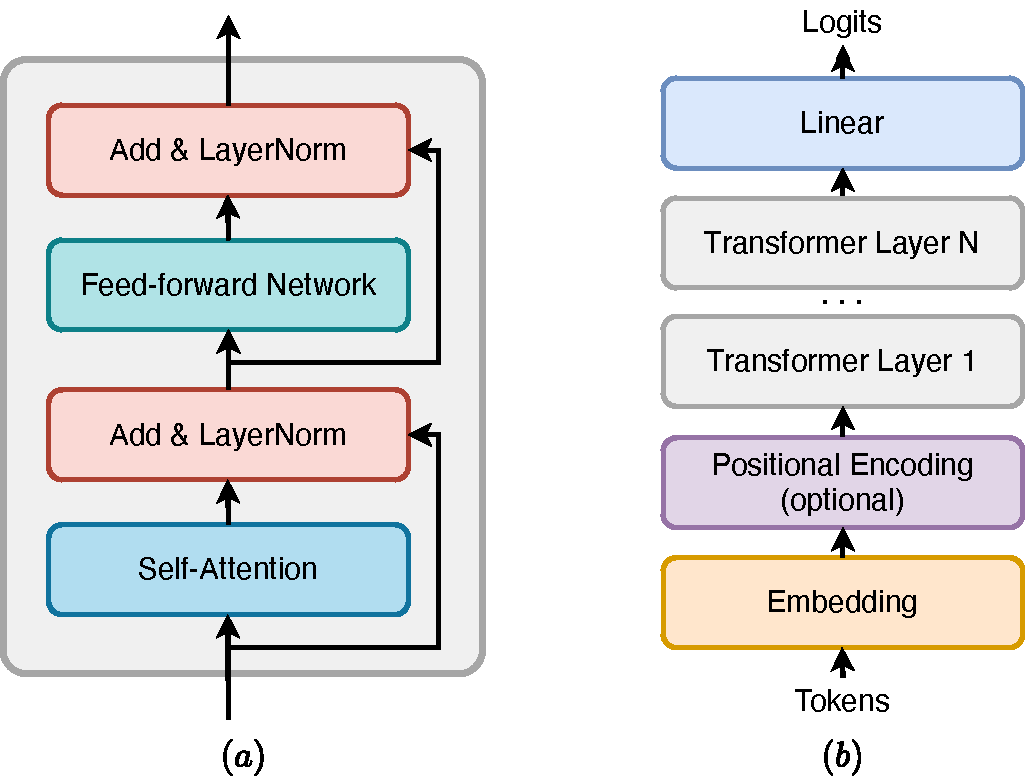
\includegraphics[width=0.8\textwidth]{fig/transformer_layer.pdf}
    \caption{(a) A single Transformer layer, consisting of multi-head self-attention, feed-forward network (MLP), and layer normalization. (b) A decoder-only transformer model. In the decoder, the self-attention mechanism has a causal mask to prevent attending to future tokens.}
    \label{fig:transformer_layer}
\end{figure}


\subsection{Encoder and Decoder Architectures}\label{subsec:types_transformers}

In this section, different Transformer architectures are summarized: encoder-decoder, encoder-only, and decoder-only models. The original Transformer~\parencite{vaswani_attention_2017} employs an encoder-decoder structure, where the encoder transforms input sequences into continuous representations, and the decoder generates output sequences based on these representations and previously generated tokens. Encoder-only models like BERT~\parencite{devlin_bert_2019} focus solely on encoding input sequences into contextual embeddings, making them well-suited for understanding tasks such as text classification and question answering. Decoder-only models, like GPT~\parencite{radford_improving_2018}, generate sequences by predicting the next token based on prior tokens, primarily used for text generation. While both encoder-decoder and decoder-only architectures can perform autoregressive sequence generation, decoder-only models are the focus of this work.

\paragraph{Encoder-Decoder}
The original Transformer model introduced by Vaswani et al.~\cite{vaswani_attention_2017} employs an encoder-decoder architecture. In this architecture, the encoder processes an input sequence $\mathbf{x} = (x_1, x_2, \dots, x_n)$ into a sequence of continuous representations $\mathbf{z} = (z_1, z_2, \dots, z_n)$. The decoder then generates an output sequence $\mathbf{y} = (y_1, y_2, \dots, y_m)$ by predicting the next token $y_t$ based on the encoder's output and the previously generated tokens.

The encoder consists of a stack of $N$ identical layers, each containing two sub-layers: a multi-head self-attention mechanism and a position-wise fully connected feed-forward network. The decoder has a similar structure but includes a third sub-layer: the \emph{cross-attention}, also called \emph{encoder-decoder attention}, where the queries come from the previous decoder layer, and the keys and values come from the output of the encoder. Hence, the difference between the self-attention and cross-attention mechanisms is that self-attention is usually applied to the same sequence, while cross-attention is applied between two different sequences (e.g. one from the encoder, and one from the decoder). Moreover, the self-attention mechanism in the decoder has a causal mask to prevent attending to ``future tokens'', ensuring output is generated autoregressively. The T5 model \parencite{raffel_exploring_2020} is an example of a large encoder-decoder Transformer model capable of performing many NLP tasks such as translation, summarization, and question answering.

\paragraph{Encoder-only}
Encoder-only models focus exclusively on encoding the input sequence into a contextual representation without a decoder component. BERT (Bidirectional Encoder Representations from Transformers)~\cite{devlin_bert_2019} is a prominent example of this architecture. BERT utilizes a stack of Transformer encoder layers to produce deep bidirectional representations by jointly conditioning on both left and right context. This makes encoder-only models particularly well-suited for tasks that require a comprehensive understanding of the input, such as text classification, named entity recognition, and question answering.

These models are typically pre-trained on large unlabeled text corpora using self-supervised objectives like masked language modeling (MLM) and next sentence prediction (NSP). The pre-trained models can then be fine-tuned on specific downstream tasks.

\paragraph{Decoder-only}
Decoder-only models generate sequences based on prior tokens and are designed primarily for autoregressive language modeling and text generation tasks. GPT (Generative Pre-trained Transformer)~\cite{radford_improving_2018} is a canonical example of a decoder-only architecture. In these models, the Transformer decoder predicts the next token in a sequence by attending to the previous tokens without an encoder component. The encoder is not needed since in a decoder-only Transformer, the input sequence $\mathbf{x}$ is prepended to the decoder input sequence $\mathbf{y}$, and only passed through the decoder layers to autoregressively generate the output sequence. Recent research on language modeling has mostly focused decoder-only models, since they can also be used on other language tasks through prompting, few-shot learning, and fine-tuning. In particular, majority of the latest state-of-the-art large language models (LLMs) are decoder-only transformers pre-trained on large text corpora.

\paragraph{Encoder-Decoder vs. Decoder-Only} Both model types are capable of autoregressive sequence generation and can be used for a wide range of tasks. The decoder-only models are favored in recent works due to them being simpler and having less inductive bias. However, encoder-decoder models are still widely used in machine translation, robotics, and multi-modal learning tasks. The additional structure in encoder-decoder models, as compared to using a decoder-only model with would-be encoder input sequence prepended to the decoder's input can be summarized as:
\begin{itemize}
    \item The input to the encoder passes through more layers (encoder layers) before reaching the decoder.
    \item It is assumed that input and output sequences are sufficiently different to justify using separate parameters for them (encoder and decoder).
\end{itemize}

With large language models and massive datasets, the difference between the two architecture becomes less relevant. In summary, the choice of Transformer architecture depends on the specific requirements of the task, though decoder-only models have been more widely used in recent research and are the focus of this work.

\subsection{Recurrent and Looping Architectures}\label{subsec:recurrent_looping}

Multiple Transformer extensions have been proposed that incorporate iterative application of weight-sharing layers, particularly suitable for algorithmic tasks that require reasoning over sequences. The Universal Transformer and Looped Transformer are two such examples that introduce recurrence into the Transformer architecture. There are other modifications the Transformer architecture, a few examples of which include the Memory Transformer \parencite{burtsev_memory_2021}, Recurrent Memory Transformer \parencite{bulatov_recurrent_2022}, and Neural Data Router \parencite{csordas_neural_2021}, but these architectures are not widely adopted in pretrained language models, and are not tested in this work.

\paragraph{Universal Transformer}
The Universal Transformer \parencite{dehghani_universal_2018} introduces recurrence into the Transformer architecture by repeatedly applying the same transformer layers multiple times, in both encoder and decoder parts:
\begin{equation*}
    H^{(t+1)} = \text{TransformerLayer}(H^{(t)}),
\end{equation*}
where $t$ denotes the iteration step. An adaptive computation time (ACT) mechanism is used to dynamically adjust the number of iterations based on the input sequence. The Universal Transformer has been shown to achieve better performance on algorithmic tasks compared to the original Transformer. It is also an interesting extension of the Transformer architecture from theoretical point of view, since it makes the model Turing-complete under certain conditions \parencite{dehghani_universal_2018}.

\begin{figure}[h!]
    \centering
    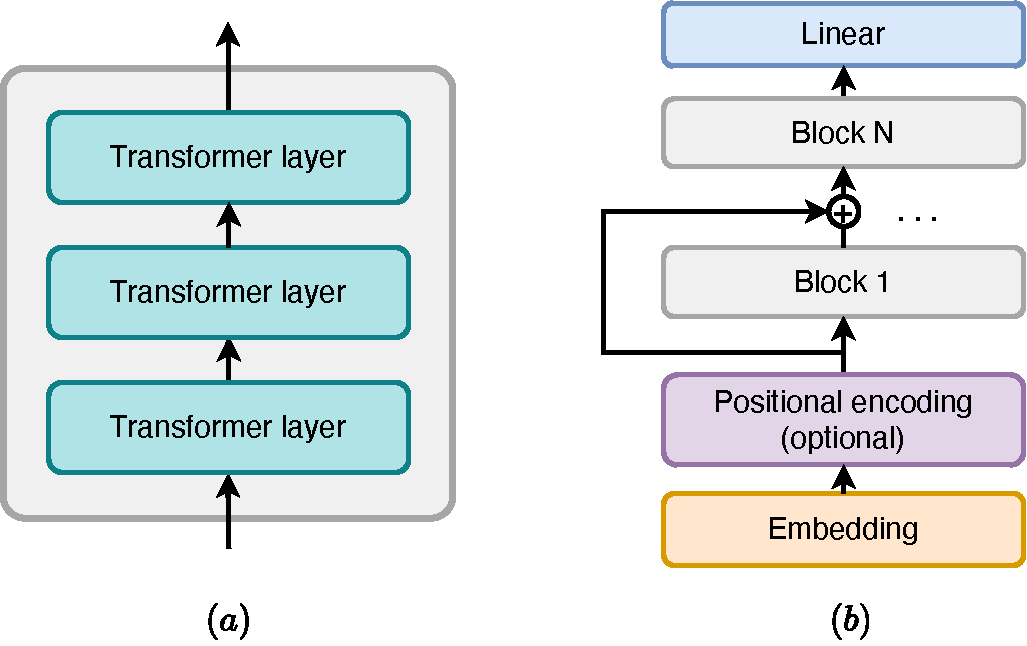
\includegraphics[width=0.8\textwidth]{fig/looped_transformer.pdf}
    \caption{(a) A block of multiple transformer layers used in the looped transformer. (b) Looped decoder-only transformer architecture. The input injection mechanism adds skip connections (arrow around blocks) from the original input sequence to the input of each block.}
    \label{fig:looped_transformer}
\end{figure}

\paragraph{Looped Transformer}
Similar to the Universal Transformer, the Looped Transformer \parencite{yang_looped_2023} extends the Transformer by incorporating iterative application of a block of transformer layers. This modification has been shown to perform better than the original, non-recurrent Transformer on algorithmic tasks \parencite{csordas_systematic_2023,yang_looped_2023}. In particular, looped transformer achieves better length generalization on the binary addition task as shown by \cite{fan_looped_2024}. The looped decoder-only transformer architecture is illustrated in Figure \ref{fig:looped_transformer}. However, unlike the Universal Transformer, the Looped Transformer is not necessarily encoder-decoder, and might not use the adaptive computation time mechanism.

\subsection{Positional Encoding Schemes}\label{subsec:positional_encoding}

Since the Transformer lacks inherent sequential order, positional encodings are added to input embeddings to provide position information. Though, several recent works have shown that the causal attention mechanism in a decoder-only transformer can also implicitly learn to encode positional information in the absence of explicit positional encodings \parencite{haviv_transformer_2022,zuo_breaking_2024,zhou_transformers_2024}. Positional encoding methods are also crucial for algorithmic tasks, especially multi-digit integer addition \parencite{shen_positional_2023,kazemnejad_impact_2023,ruoss_randomized_2023}

\paragraph{Absolute Positional Encoding}\label{subsec:absolute_pos_enc}
The original Transformer \parencite{vaswani_attention_2017} uses additive vectors of same dimensionality as the embeddings to encode the \emph{absolute} positions of the tokens. These vectors could be learned (from a random initialization), or \emph{sinusoidal}, where the latter are defined as:
\begin{align*}
    \mathbf{p}_{i,2k}   & = \sin\left( \frac{i}{10000^{2k/d}} \right), \\
    \mathbf{p}_{i,2k+1} & = \cos\left( \frac{i}{10000^{2k/d}} \right),
\end{align*}
for position in the sequence $i$ and dimension $k$. In \cite{vaswani_attention_2017}, the performance difference between learned and sinusoidal positional encodings was found to be insignificant, and the use of sinusoidal encodings is justified by possibility of generalization to longer sequences. In practice, however, absolute positional encodings do not generalize well to sequences longer than the ones seen during training \parencite{press_train_2021}.

\paragraph{Randomized Positional Encodings}\label{subsec:random_pos_enc}
Randomized positional encodings \cite{ruoss_randomized_2023} aim to improve length generalization by simulating longer sequences during training. Similarly to absolute positional encodings, they are added to the input embeddings, and have separate vectors for each position in the sequence. However, instead of using sequential positions $1, 2, \dots, n$, the positions are randomly sampled (keeping order) from a range $[1, n_{\text{max}}]$, where $n_{\text{max}}$ is the maximum sequence length. Thus, the model is exposed to a wider range of positional encodings during training, which helps improve generalization to longer sequences. A related method is to randomly insert spaces between tokens in the input sequence (e.g. \texttt{123 + 456} might become \texttt{12 3  + 45 6}), which disrupts the model's dependence on absolute position information and encourages it to learn more robust representations \parencite{shen_positional_2023}. It is important to distinguish this method from the one introduced by \cite{shen_positional_2023} named Random Embedding, where a random Gaussian ``tag'' is added to a subset of embedding dimensions.

\paragraph{Relative Position Encoding}\label{subsec:relative_pos_enc}
Relative position representations \parencite{shaw_self-attention_2018} encode the relative distances between sequence elements directly into the attention mechanism. In RPE, a vector $\mathbf{a}_{i, j} \in \mathbb{R}^d$ is learned for each pair of positions $(i, j)$, and added to the keys before computing the attention scores:
\begin{equation*}
    A_{ij} = \frac{\mathbf{q}_i (\mathbf{k}_i + \mathbf{a}_{ij}^K)^\top}{\sqrt{d}}
\end{equation*}
where $\mathbf{q}_i$ and $\mathbf{k}_j$ are the query and key vectors for positions $i$ and $j$, respectively. Relative position encodings have been shown to improve performance on tasks requiring long-range dependencies \parencite{shaw_self-attention_2018}.

\paragraph{Attention with Linear Biases (ALiBi)}\label{subsec:alibi}
ALiBi~\parencite{press_train_2021} introduces a linear bias to the attention scores based on the relative positions. For this additive method, the computation of the (pre-softmax) attention logits is modified as:
\begin{equation*}
    A_{\text{ALiBi}}(X) = Q K^\top + B,
\end{equation*}
where the bias matrix $B \in \mathbb{R}^{n \times n}$ is computed by the position encoding function $b : \mathbb{N}^2 \to \mathbb{R}$, such that the $(i,j)$-th entry of $B$ is $b(i,j)$. The bias function for the relative position encoding is defined as:
\begin{equation*}
    b(i,j) = -r|i - j|
\end{equation*}
where the $r$ is a fixed slope pre-computed for each head.

\paragraph{Rotary Position Encoding (RoPE)}\label{subsec:rope}
RoPE \cite{su_roformer_2024} encodes positions using rotations of the query and key vectors with an angle proportional to their absolute positions before the dot product attention, which results in attention being a function of the relative distance between the tokens, capturing the relative positional information. It is a non-additive relative positional encoding. Works such as \cite{press_train_2021,kazemnejad_impact_2023} show that RoPE also has poor length generalization in addition tasks.

\subsection{Training and Inference}\label{subsec:training_inference}

\begin{figure}[h!]
    \centering
    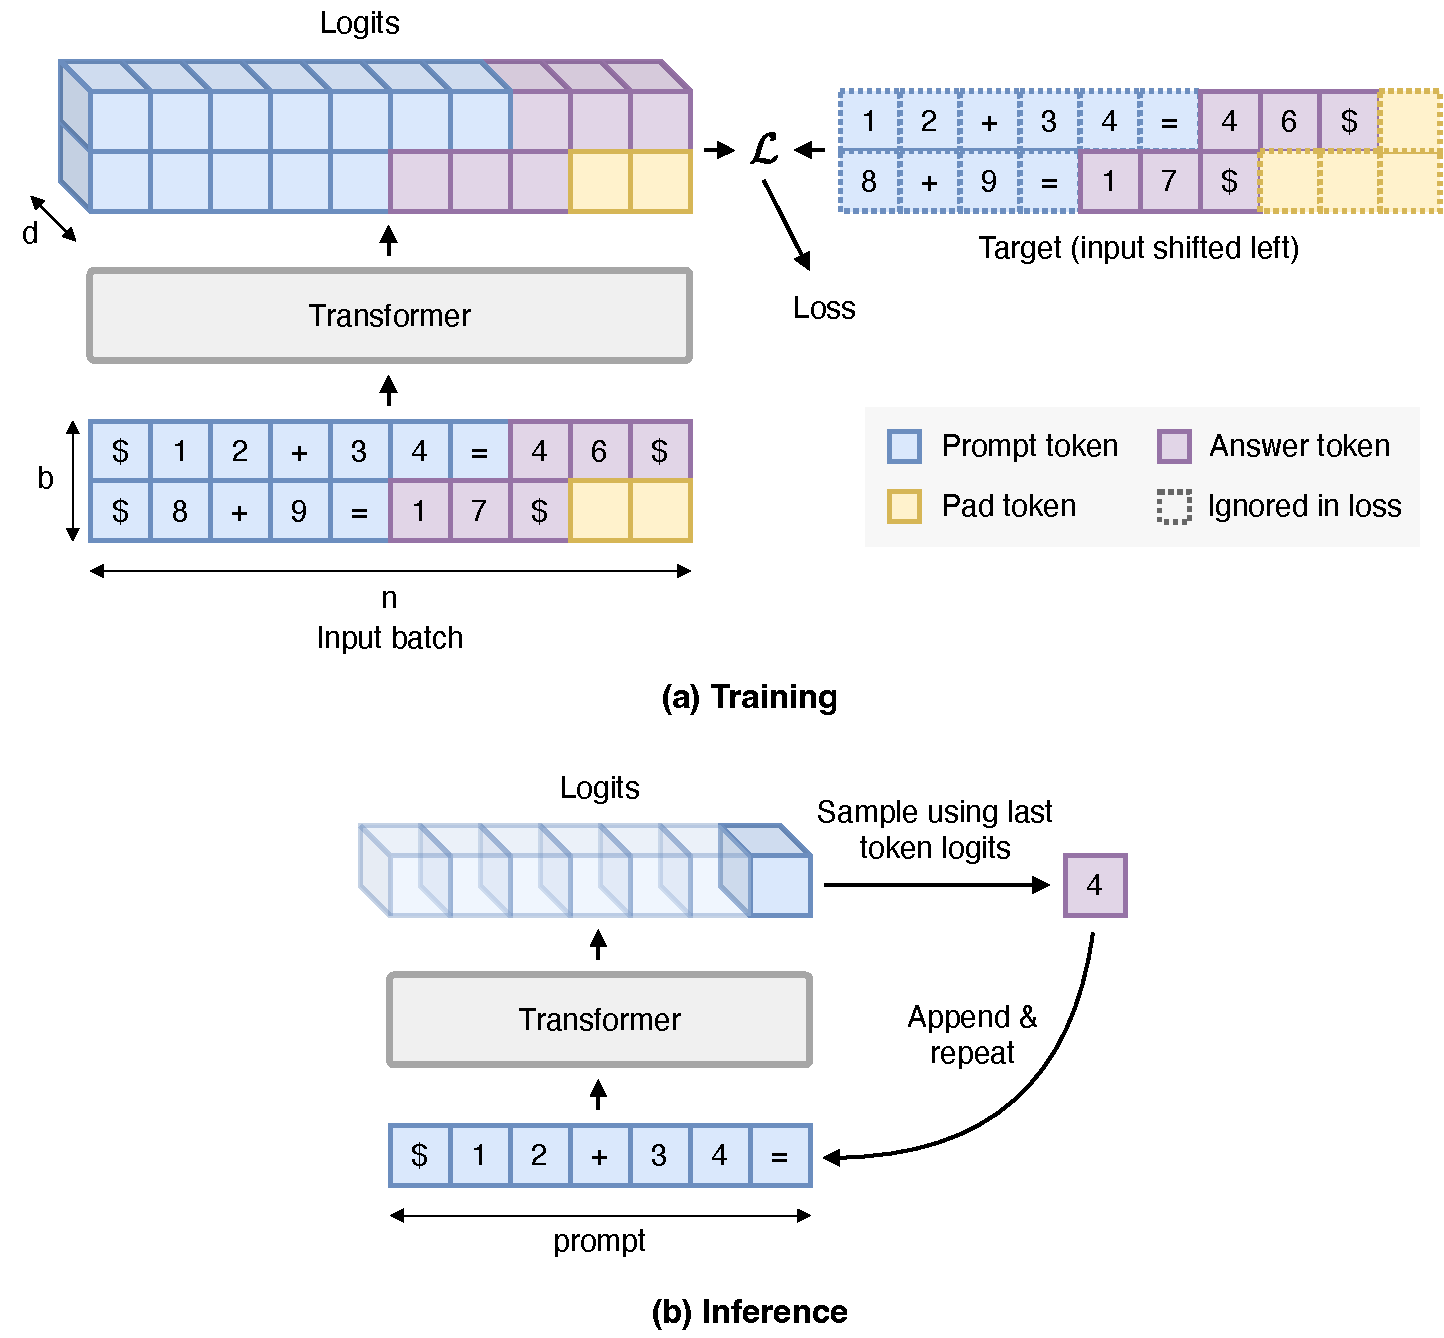
\includegraphics[width=0.9\textwidth]{fig/training_and_inference.pdf}
    \caption{Training and inference setup for Transformer models on the arithmetic task. During training (subfigure a), the padded input batch is passed through the model, and the loss is computed by comparing the predicted logits with the target sequence (\emph{teacher forcing}). Unlike regular unsupervised learning, the loss from non-answer tokens is masked out in experiments. During inference (subfigure b), the model generates outputs by greedily sampling tokens one by one until maximum output length is reached, or the end-of-sequence token \texttt{\$} is generated.}
    \label{fig:transformer_training_inference}
\end{figure}

\paragraph{Training}
Training involves minimizing a loss function, typically the \emph{cross-entropy loss} for language tasks, using an optimization algorithm like Stochastic Gradient Descent (SGD) or AdamW~\parencite{loshchilov_decoupled_2018}. The model learns the parameters $\theta$ by backpropagating the loss through the network layers. The cross-entropy loss is defined as:
\begin{equation*}
    \mathcal{L} = -\frac{1}{b} \sum_{i=1}^{b} \sum_{j=1}^{n} \log p(x_{i,j} | x_{i,<j}),
\end{equation*}
where $b$ is the batch size, $n$ is the sequence length, and $p(x_{i,j} | x_{i,<j})$ is the probability of token $x_{i,j}$ given the previous tokens $x_{i,<j}$.

\paragraph{Answer Loss Masking}
For tasks like integer addition, the loss is modified to focus only on the answer tokens, where a binary mask \( m_{i,j} \in \{0, 1\} \) is applied to denote whether a token at position \( j \) in sequence \( i \) corresponds to an answer. The loss becomes:

\begin{equation*}
    \mathcal{L}_{\text{answer-only}} = -\frac{1}{b} \sum_{i=1}^{b} \sum_{j=1}^{n} m_{i,j} \log p(x_{i,j} | x_{i,<j}),
\end{equation*}

where $b$ is the batch size, $n$ is the sequence length, $m_{i,j} = 1$ if token \( x_{i,j} \) is an answer token, otherwise \( m_{i,j} = 0 \), and \( p(x_{i,j} | x_{i,<j}) \) is the predicted probability of token \( x_{i,j} \) given the preceding tokens \( x_{i,<j} \).

This formulation ensures that the loss is computed only over the answer tokens, with non-answer tokens effectively ignored (since \( m_{i,j} = 0 \) for those positions). Without answer loss masking, the cross-entropy loss would penalize the model for incorrectly predicting randomly generated operands as well (which are not possible to predict in the first place), thus adding noise to the training process never reaching 0 loss.

\paragraph{Inference}
During inference, the trained model generates outputs by iteratively computing the forward pass through the network and adding the sampled tokens to the prompt sequence each time. In autoregressive models, tokens are generated one by one, conditioned on previous outputs. The token at each step is selected using \emph{greedy sampling}, where:
\begin{equation*}
    x_j = \arg\max_{x \in \mathcal{V}} p_{\theta}(x | x_{<j}),
\end{equation*}
where $\mathcal{V}$ is the vocabulary, $p_{\theta}(x | x_{<j})$ are the logits computed by the model, and $\text{softmax}$ is applied to obtain the probabilities from non-normalized logits. The input sequence for the next step is updated by appending the predicted token to the previous sequence:
\begin{equation*}
    x^{t+1} = [x^t, x_j].
\end{equation*}
The sampling process continues until a predefined stopping criterion is met, such as reaching a maximum sequence length or generating a special end-of-sequence token. Greedy sampling is computationally efficient but does not explore alternative sequences. However, it is sufficient for tasks like integer addition, where the output is deterministic.


\section{Mechanistic Interpretability}\label{sec:mech_interp}

Understanding how Transformers make decisions is crucial for interpretability and debugging. Relevant concepts include the \emph{residual stream}, \emph{activation patching}, and the \emph{logit lens}, which provide insights into the model's internal representations and decision-making processes.

\paragraph{Residual Stream}
The residual stream in a Transformer is enabled by the residual connections around operations (as described in Subsection \ref{subsec:elements_transformers}) and serves as a shared memory, accumulating information across layers via residual connections. Both attention heads and feedforward layers read from and write to this stream, which ensures the propagation of information throughout the model. Since each layer can only read from earlier layers, analyzing this stream is essential for understanding how information is transformed and stored across layers \parencite{elhage2021mathematical}. The residual stream can be studied by techniques such as activation patching to trace information flow.

\paragraph{Circuits}
Circuits in Transformers are a set of elements (i.e. attention heads, feed-forward layers) that are responsible for specific behaviors. Currently, while multiple methods exist that attempt to discover circuits, there is no structured way to identify all circuits of interest, nor is it certain that human-interpretable circuits exist in the first place in any given model \parencite{ferrando_primer_2024}. Some works succeeded in identifying specific high-level circuits such as ones performing modular addition \parencite{nanda_progress_2022,zhong_clock_2023} and indirect object identification \parencite{wang_interpretability_2022}. Discovering and explaining circuits is helpful for learning algorithmic tasks and compositionality, like multi-digit integer addition. For instance, a number of circuits might emerge in the model that perform the sub-tasks for integer addition (such as digit-wise modular addition, and carry propagation), and the answer might be generated by composing their outputs.

% \paragraph{Activation Patching}
% Activation patching \parencite{zhang_towards_2023} is a causal analysis technique where activations from a run of the model are replaced by activations from a different context, allowing to observe how this change affects the model's predictions. By selectively patching different layers or tokens, it becomes possible to identify which parts of the model are responsible for specific behaviors, such as copying repeated sequences or in-context learning. For instance, patching activations in the residual stream can reveal the contribution of circuits like \emph{induction heads}, which are attention heads that predict repeated sequences \parencite{olsson_-context_2022}.

\section{Expressivity}\label{sec:expressivity}

In the context of Transformers, expressivity refers to whether a given task or behavior can be reliably implemented using the model's learned representations. One framework for analyzing this is \emph{RASP}, a restricted-access sequence processing language \parencite{weiss_thinking_2021} that mimics the operations of transformers in a more interpretable manner. Moreover, \cite{fan_looped_2024} show using RASP that looped transformers can generalize to longer sequence lengths for binary addition task, along with other algorithmic tasks.

A key aspect of Transformers is their ability to generalize \emph{compositionally} in some tasks, as highlighted by \cite{hupkes_compositionality_2020}. This suggests that, under the right conditions, transformers are capable of learning systematic combinations of components, enabling them to generalize beyond seen examples in a structured manner. This compositional behavior is crucial for algorithmic tasks, where the model must apply learned rules consistently across different sequence lengths. However, it is not clear how it can be proven that a Transformer model of specific architecture and size can learn a particular task, especially for complex tasks like multi-digit integer addition.

\TODO{discuss \cite{zhou_what_2023}, show addition algo in RASP-L, but with limits: index hints, padding ops to same digit length}

\section{Deep Double Descent}\label{sec:deep_double_descent}

The phenomenon of \emph{deep double descent} describes how increasing model capacity or training duration can initially lead to worse generalization before ultimately improving it. This was initially believed to challenge the traditional bias-variance tradeoff, where increasing model complexity was believed to always result in overfitting \parencite{belkin_reconciling_2019, nakkiran_deep_2021}. Deep double descent arises when models, especially overparameterized ones, first memorize the training data, but later discover more generalizable features, leading to improved performance on the test set and zero training loss.

This phenomenon is still relevant in integer addition tasks, since the interpolation threshold — the point where the model transitions from memorization to generalization might change with respect to model and dataset size.

\cleardoublepage

\chapter{State of the Art}\label{sota}


\cleardoublepage

\chapter{Research Questions}\label{research_questions}


\section*{Research Questions}

\begin{enumerate}
    \item How do (smaller) transformers learn to compose sub-tasks for integer addition?
    \item What architectural features or training strategies enhance compositional learning? (we want them to be applicable to other domains as well, at least not hurt in regular unsupervised text setting)
    \item How do transformers generalize to larger sequences than seen during training?
\end{enumerate}

Compositionality gap: difference between performance on subtasks and the full task. In our case full task is integer addition, with subtasks being digit-wise alignment, addition, and carry operations.

\subsection*{Experiments / Hypotheses}

\begin{itemize}
    \item RQ3: Models generalize to in-distribution sequence lengths but not OOD (longer or shorter) lengths.
          \begin{itemize}
              \item Baseline performance.
              \item Smaller $3 \times 3$, $7 \times 7$ experiments, 1-19 digits and 18/20+ digits
              \item Scratchpad can improve it to 18 and 20, not 21+
          \end{itemize}

    \item RQ1: Sub-task decomposition: models decompose addition into:
          \begin{itemize}
              \item digit-wise alignment
              \item modular digit-wise addition
              \item carry operations
              \item Probing tasks for sub-task neural networks, saliency, etc. (TODO)
          \end{itemize}

    \item RQ2: Positional embeddings are important for digit-wise addition and source of errors (e.g., alignment).
          \begin{itemize}
              \item Random spaces
              \item Abacus
              \item Relative pos encodings
          \end{itemize}

    \item RQ1: Compositional learning strategies:
          \begin{itemize}
              \item Simple to complex tasks (curriculum)
              \item Multi-task learning (aux loss) (TODO)
          \end{itemize}

    \item Error analysis: TODO for robustness.

\end{itemize}

\cleardoublepage

\chapter{Approach}\label{approach}
\cleardoublepage

\chapter{Conclusion}\label{conclusion}
\cleardoublepage

%%%%%%%%%%%%%%%%%%%%%%%%%%%%
% Appendices:
% these are optional! For most Bachelor-theses and some Master-thesis none of them is needed. 
% Just comment them if not needed.
\appendix
\fancyhead[LO,RE]{}                      % Define the header style for the appendixpages

\fancyhead[LE,RO]{\it Appendix A. Nomenclature}                %Adapt letter!
\chapter{Nomenclature}\label{app:nomenclature}

\begin{table}[H]
    \centering
    \begin{tabular}{ll}
        \toprule
        \textbf{Symbol} & \textbf{Description}                                    \\
        \midrule
        SOTA            & State-of-the-art                                        \\
        MLP             & Multi-layer perceptron                                  \\
        SGD             & Stochastic gradient descent                             \\
        FFNN            & Feed-forward neural network                             \\
        RNN             & Recurrent neural network                                \\
        GPT             & Generative pre-trained transformer                      \\
        BERT            & Bidirectional encoder representations from transformers \\
        T5              & Text-to-text transfer transformer                       \\
        LLM             & Large language model                                    \\
        CoT             & Chain-of-thought                                        \\
        OOD             & Out-of-distribution                                     \\
        \bottomrule
    \end{tabular}
    \caption{Table of nomenclature}
    \label{tab:nomenclature}
\end{table}
\cleardoublepage

% ... add as much appendices as you need (one can also add source code, for example)

%\fancyhead[LE]{\it \leftmark}
%\chapter{}
\fancyhead[LE,RO]{\it Bibliography}       % A bibliography never have a letter or numbering!
% \bibliographystyle{plain}             % Style for presenting the literature
\phantomsection\addcontentsline{toc}{chapter}{Bibliography}% Add to the TOC
% \bibliography{thesis}
\printbibliography
\cleardoublepage

%%%%%%%%%%%%%%%%%%%%%%%%%%%%
% Formal page 1
\vspace{2cm}
\chapter*{Erkl\"arung der Urheberschaft}
\label{sec:urheber}
\fancyhead[LE]{\it Erkl\"arung der Urheberschaft}
Hiermit versichere ich an Eides statt, dass ich die vorliegende
\trtype{} im Studiengang \trcourseofstudies{}
selbstst{\"a}ndig verfasst und keine anderen als die angegebenen
Hilfsmittel - insbesondere keine im Quellenverzeichnis nicht
benannten Internet-Quellen – benutzt habe. Alle Stellen, die
w{\"o}rtlich oder sinngem{\"a}{\ss} aus Ver{\"o}ffentlichungen entnommen wurden,
sind als solche kenntlich gemacht. Ich versichere weiterhin, dass
ich die Arbeit vorher nicht in einem anderen Pr{\"u}fungsverfahren
eingereicht habe und die eingereichte schriftliche Fassung der
auf dem elektronischen Speichermedium entspricht.

\vspace{4cm}
\noindent Ort, Datum \hfill Unterschrift

%The backcover is always empty
\newpage
\thispagestyle{empty}
\hspace{1cm}
\newpage

%%%%%%%%%%%%%%%%%%%%%%%%%%%%
% Formal page 2
\vspace{2cm}
\chapter*{Erkl\"arung zur Ver\"offentlichung}
\label{sec:erklaerung}
\fancyhead[LE]{\it Erkl\"arung zur Ver\"offentlichung}
Ich stimme der Einstellung der \trtype{} in die Bibliothek des Fachbereichs Informatik zu.

\vspace{4cm}
\noindent Ort, Datum \hfill Unterschrift

%The backcover is always empty
\newpage
\thispagestyle{empty}
\hspace{1cm}
\newpage

\end{document}
%EOF

